\documentclass[a4paper,11pt]{article}

\usepackage{préambule}

\title{Chapitre 3 : Symétrie}
\date{}
\author{}

\begin{luacode}
dofile "symetrie.lua"
\end{luacode}

\begin{document}

\maketitle

\section{Symétrie axiale}

\begin{cours}
	On dit que deux figures sont \textbf{symétriques par rapport à une droite} (appelée \textbf{l'axe de symétrie}) si elles se superposent quand on plie le long de cette droite.
\end{cours}

\begin{exemple}
	\begin{tikzpicture}
		\directlua{
		local axis = {
				p1 = {x = 3.8, y = 2},
				p2 = {x = 3.8, y = 6},
			}
		local points = {
		{x = 2, y = 5},
		{x = 2, y = 4},
		{x = 1, y = 4},
		{x = 1.5, y = 3.5},
		{x = 2.5, y = 3.5},
		{x = 3, y = 4},
		{x = 2, y = 4},
		{x = 2, y = 4.2},
		{x = 1.2, y = 4.2},
		{x = 2, y = 5},
		}
		points_symetriques = symetrie_axiale(axis, points)
		tikz_draw_points(points)
		tikz_draw_points(points_symetriques)
		draw_axis(axis, nil)
		tikz_draw_points({points[6], points_symetriques[6]}, "dashed")
		}
		\node[color=red] at (5.6, 3) {Axe de symétrie};

		\draw[black,thick] (3.8,4.2) -- ++(0.2,0) -- ++(0,-0.2);

		\draw[black,thick] (3.3,4.1) -- ++(0.2,-0.2);
		\draw[black,thick] (3.4,4.1) -- ++(0.2,-0.2);

		\draw[black,thick] (4.15,4.1) -- ++(0.2,-0.2);
		\draw[black,thick] (4.25,4.1) -- ++(0.2,-0.2);
	\end{tikzpicture}
\end{exemple}

\begin{exemple}
	\begin{tikzpicture}
		\directlua{
		local axis = {
				p1 = {x = 3, y = 2},
				p2 = {x = 5, y = 6},
			}
		local head = {
		{x = 0.8, y = 4.4},
		{x = 1, y = 5},
		{x = 1.05, y = 5},
		{x = 1.2, y = 5.4},
		{x = 1.35, y = 5},
		{x = 1, y = 5},
		{x = 2.35, y = 5},
		{x = 2.2, y = 5.4},
		{x = 2.05, y = 5},
		{x = 2.4, y = 5},
		{x = 2.6, y = 4.4},
		{x = 2, y = 3.8},
		{x = 1.4, y = 3.8},
		{x = 0.8, y = 4.4},
		}
		local nose = {
		{x = 1.7, y = 4.3},
		{x = 1.8, y = 4.4},
		{x = 1.6, y = 4.4},
		{x = 1.7, y = 4.3},
		}
		local mustache1 = {
		{x = 1.8, y = 4.3},
		{x = 2, y = 4.1},
		}
		local mustache2 = {
		{x = 1.82, y = 4.34},
		{x = 2.04, y = 4.2},
		}
		local mustache3 = {
		{x = 1.6, y = 4.3},
		{x = 1.4, y = 4.1},
		}
		local mustache4 = {
		{x = 1.58, y = 4.34},
		{x = 1.36, y = 4.2},
		}
		local head_symetrique = symetrie_axiale(axis, head)
		tikz_draw_points(head)
		tikz_draw_points(nose)
		tikz_draw_points(mustache1)
		tikz_draw_points(mustache2)
		tikz_draw_points(mustache3)
		tikz_draw_points(mustache4)
		tikz_draw_points(head_symetrique)
		tikz_draw_points(symetrie_axiale(axis, nose))
		tikz_draw_points(symetrie_axiale(axis, mustache1))
		tikz_draw_points(symetrie_axiale(axis, mustache2))
		tikz_draw_points(symetrie_axiale(axis, mustache3))
		tikz_draw_points(symetrie_axiale(axis, mustache4))
		draw_axis(axis, "west")
		tikz_draw_points({head[11], head_symetrique[11]}, "dashed")
		}
		\draw[black,thick,rotate around={62.5:(4,4)}] (3.73,4.2) -- ++(0.2,0) -- ++(0,-0.2);

		\draw[black,thick] (3.2,4.23) -- ++(0.1,-0.3);
		\draw[black,thick] (3.3,4.2) -- ++(0.1,-0.3);

		\draw[black,thick] (4.5,3.59) -- ++(0.1,-0.3);
		\draw[black,thick] (4.6,3.56) -- ++(0.1,-0.3);
	\end{tikzpicture}
\end{exemple}


\begin{methode}
	% Takes 'point_x', 'axis_x'
	\newcommand\mySymetricToAxis[2]{
		\directlua{
			local arg1 = token.scan_argument()
			local arg2 = token.scan_argument()
			tex.print(2 * tonumber(arg2) - tonumber(arg1))
		}
		{#1}{#2}
	}
	Pour faire le symétrique par rapport à un axe :
	\begin{enumerate}
		\item Pour chaque point sur la figure d'origine, trace une ligne passant par ce point, \textbf{perpendiculaire} à l'axe de symétrie.

		      \newcommand{\Ax}{0}
		      \newcommand{\Ay}{2}
		      \newcommand{\Bx}{1}
		      \newcommand{\By}{1}
		      \newcommand{\Cx}{0}
		      \newcommand{\Cy}{0}

		      \newcommand{\mycoordinates}{
			      \coordinate (A) at (\Ax,\Ay);
			      \coordinate (B) at (\Bx,\By);
			      \coordinate (C) at (\Cx,\Cy);
			      \coordinate (A_mid) at (3,\Ay);
			      \coordinate (B_mid) at (3,\By);
			      \coordinate (C_mid) at (3,\Cy);
			      \coordinate (A') at (\mySymetricToAxis{\Ax}{3},\Ay);
			      \coordinate (B') at (\mySymetricToAxis{\Bx}{3},\By);
			      \coordinate (C') at (\mySymetricToAxis{\Cx}{3},\Cy);
		      }

		      \begin{tikzpicture}
			      \mycoordinates

			      \draw[fill=gray] (A) circle (2pt) node[anchor=south east] {A};
			      \draw[fill=gray] (B) circle (2pt) node[anchor=south west] {B};
			      \draw[fill=gray] (C) circle (2pt) node[anchor=south east] {C};
			      \draw (A) -- (B);
			      \draw (B) -- (C);
			      \draw[color=red] (3,-1) -- (3,3);

			      \draw[dashed] (-1,\Ay) -- (7,\Ay);

			      \draw ([xshift=-0.2cm] A_mid) -- ++(0,0.2) -- ++(0.2,0);
		      \end{tikzpicture}
		\item Puis, place un point \textbf{à la même distance} de l'autre côté de l'axe.

		      \begin{tikzpicture}
			      \mycoordinates

			      \draw[fill=gray] (A) circle (2pt) node[anchor=south east] {A};
			      \draw[fill=gray] (B) circle (2pt) node[anchor=south west] {B};
			      \draw[fill=gray] (C) circle (2pt) node[anchor=south east] {C};
			      \draw (A) -- (B);
			      \draw (B) -- (C);
			      \draw[color=red] (3,-1) -- (3,3);

			      \draw[dashed] (-1,\Ay) -- (7,\Ay);

			      \draw ([xshift=-0.2cm] A_mid) -- ++(0,0.2) -- ++(0.2,0);

			      \draw (1.4,2.2) -- (1.6,1.8);
			      \draw (4.3,2.2) -- (4.5,1.8);

			      \draw[fill=gray] (A') circle (2pt) node[anchor=south west] {A'};
		      \end{tikzpicture}
		\item Fait de même pour les autres point :

		      \begin{tikzpicture}
			      \mycoordinates

			      \draw[fill=gray] (A) circle (2pt) node[anchor=south east] {A};
			      \draw[fill=gray] (B) circle (2pt) node[anchor=south west] {B};
			      \draw[fill=gray] (C) circle (2pt) node[anchor=south east] {C};
			      \draw (A) -- (B);
			      \draw (B) -- (C);
			      \draw[color=red] (3,-1) -- (3,3);

			      \draw[dashed] (-1,\Ay) -- (7,\Ay);
			      \draw[dashed] (-1,\By) -- (7,\By);
			      \draw[dashed] (-1,\Cy) -- (7,\Cy);

			      \draw ([xshift=-0.2cm] A_mid) -- ++(0,0.2) -- ++(0.2,0);
			      \draw ([xshift=-0.2cm] B_mid) -- ++(0,0.2) -- ++(0.2,0);
			      \draw ([xshift=-0.2cm] C_mid) -- ++(0,0.2) -- ++(0.2,0);

			      \draw (1.4,2.2) -- (1.6,1.8);
			      \draw (4.3,2.2) -- (4.5,1.8);

			      \draw (2,1.2) -- (2.2,0.8);
			      \draw (2.1,1.2) -- (2.3,0.8);
			      \draw (3.7,1.2) -- (3.9,0.8);
			      \draw (3.8,1.2) -- (4,0.8);

			      \draw (1.2,0.2) -- (1.4,-0.2);
			      \draw (1.3,0.2) -- (1.5,-0.2);
			      \draw (1.4,0.2) -- (1.6,-0.2);
			      \draw (4.3,0.2) -- (4.5,-0.2);
			      \draw (4.4,0.2) -- (4.6,-0.2);
			      \draw (4.5,0.2) -- (4.7,-0.2);

			      \draw[fill=gray] (A') circle (2pt) node[anchor=south west] {A'};
			      \draw[fill=gray] (B') circle (2pt) node[anchor=south east] {B'};
			      \draw[fill=gray] (C') circle (2pt) node[anchor=south west] {C'};
		      \end{tikzpicture}
		\item Enfin, relie les points qui étaient reliés sur la figure d'origine.

		      \begin{tikzpicture}
			      \mycoordinates

			      \draw[fill=gray] (A) circle (2pt) node[anchor=south east] {A};
			      \draw[fill=gray] (B) circle (2pt) node[anchor=south west] {B};
			      \draw[fill=gray] (C) circle (2pt) node[anchor=south east] {C};
			      \draw (A) -- (B);
			      \draw (B) -- (C);
			      \draw[color=red] (3,-1) -- (3,3);

			      \draw[dashed] (-1,\Ay) -- (7,\Ay);
			      \draw[dashed] (-1,\By) -- (7,\By);
			      \draw[dashed] (-1,\Cy) -- (7,\Cy);

			      \draw ([xshift=-0.2cm] A_mid) -- ++(0,0.2) -- ++(0.2,0);
			      \draw ([xshift=-0.2cm] B_mid) -- ++(0,0.2) -- ++(0.2,0);
			      \draw ([xshift=-0.2cm] C_mid) -- ++(0,0.2) -- ++(0.2,0);

			      \draw (1.4,2.2) -- (1.6,1.8);
			      \draw (4.3,2.2) -- (4.5,1.8);

			      \draw (2,1.2) -- (2.2,0.8);
			      \draw (2.1,1.2) -- (2.3,0.8);
			      \draw (3.7,1.2) -- (3.9,0.8);
			      \draw (3.8,1.2) -- (4,0.8);

			      \draw (1.2,0.2) -- (1.4,-0.2);
			      \draw (1.3,0.2) -- (1.5,-0.2);
			      \draw (1.4,0.2) -- (1.6,-0.2);
			      \draw (4.3,0.2) -- (4.5,-0.2);
			      \draw (4.4,0.2) -- (4.6,-0.2);
			      \draw (4.5,0.2) -- (4.7,-0.2);

			      \draw[fill=gray] (A') circle (2pt) node[anchor=west] {A'};
			      \draw[fill=gray] (B') circle (2pt) node[anchor=south east] {B'};
			      \draw[fill=gray] (C') circle (2pt) node[anchor=west] {C'};
			      \draw (A') -- (B');
			      \draw (B') -- (C');
		      \end{tikzpicture}
	\end{enumerate}
\end{methode}


\section{Symétrie centrale}

\begin{cours}
	On dit que deux figures sont \textbf{symétriques par rapport à un point} (appelée \textbf{le centre de symétrie}) si elles se superposent quand fait un demi-tour autour du point.
\end{cours}

\begin{exemple}
	\begin{tikzpicture}
		\directlua{
		local centre = { x = 5, y = 3 }
		local points = {
		{x = 2, y = 5},
		{x = 2, y = 4},
		{x = 1, y = 4},
		{x = 1.5, y = 3.5},
		{x = 2.5, y = 3.5},
		{x = 3, y = 4},
		{x = 2, y = 4},
		{x = 2, y = 4.2},
		{x = 1.2, y = 4.2},
		{x = 2, y = 5},
		}

		local points_symetrique = symetrie_centrale(centre, points)

		tikz_draw_points(points)
		tikz_draw_points(points_symetrique)
		tikz_draw_points({points[5], points_symetrique[5]}, "dashed")
		tikz_draw_points({points[6], points_symetrique[6]}, "dashed")
		draw_center(centre, "south west")
		}

		\draw[black,thick] (3.8,3.75) -- ++(0.1,-0.3);
		\draw[black,thick] (6,2.6) -- ++(0.1,-0.3);

		\draw[black,thick] (3.6,3.45) -- ++(0.1,-0.3);
		\draw[black,thick] (3.7,3.44) -- ++(0.1,-0.3);
		\draw[black,thick] (6.2,2.9) -- ++(0.1,-0.3);
		\draw[black,thick] (6.3,2.89) -- ++(0.1,-0.3);
	\end{tikzpicture}
\end{exemple}

\begin{methode}
	Pour faire le symétrique d'un point A par rapport à un centre O : \vspace{1em}

	\begin{tikzpicture}
		\coordinate (O) at (0,0);


		\draw[fill] (O) circle (2pt) node[anchor=south west] {O};
		\draw[fill] (O) ++(-1,1) circle (2pt) node[anchor=north east] {A};
	\end{tikzpicture}
	\begin{enumerate}
		\item Trace la droite, qui part du point et passe par le centre :

		      \begin{tikzpicture}
			      \coordinate (O) at (0,0);
			      \coordinate (A) at ([xshift=-1cm,yshift=1cm] O);


			      \draw[fill] (O) circle (2pt) node[anchor=south west] {O};
			      \draw[fill] (A) circle (2pt) node[anchor=north east] {A};
			      \draw[dashed] (A) ++(-0.5,0.5) -- (O) -- ++(1.5,-1.5);
		      \end{tikzpicture}
		\item Place le symétrique du point A \textbf{à égale distance de O} :

		      \begin{tikzpicture}
			      \coordinate (O) at (0,0);
			      \coordinate (A) at (-1,1);
			      \coordinate (A_sym) at (1,-1);


			      \draw[fill] (O) circle (2pt) node[anchor=south west] {O};
			      \draw[fill] (A) circle (2pt) node[anchor=north east] {A};
			      \draw[fill] (A_sym) circle (2pt) node[anchor=south west] {A'};
			      \draw[dashed] (A) ++(-0.5,0.5) -- (O) -- ++(1.5,-1.5);

			      \draw (-0.6,0.4) -- ++(0.2,0.2);
			      \draw (-0.55,0.35) -- ++(0.2,0.2);

			      \draw[rotate around={180:(O)}] (-0.6,0.4) -- ++(0.2,0.2);
			      \draw[rotate around={180:(O)}] (-0.55,0.35) -- ++(0.2,0.2);
		      \end{tikzpicture}

		      Tu peux utiliser un \textbf{compas} pour cette étape !
	\end{enumerate}
\end{methode}

\section{Propriétés de la symétrie centrale}

\begin{cours}
	Si deux droites sont symétriques par rapport à un point, alors elles sont \\ \myuline{parallèles}. \vspace{1em}

	\begin{tikzpicture}
		\coordinate (O) at (0,0);

		\draw[fill] (O) circle (2pt) node[anchor=north west] {O};

		\draw (-2,0) -- (0,1) node[anchor=south] {$(d)$} -- (2,2);
		\draw[rotate around={180:(O)}] (-2,0) -- (0,1) node[anchor=north] {$(d')$}  -- (2,2);
	\end{tikzpicture}
\end{cours}

\begin{cours}
	Le symétrique d'un segment par rapport à un point a la même longueur : \myuline{la symétrie conserve les longueurs}. \vspace{1em}

	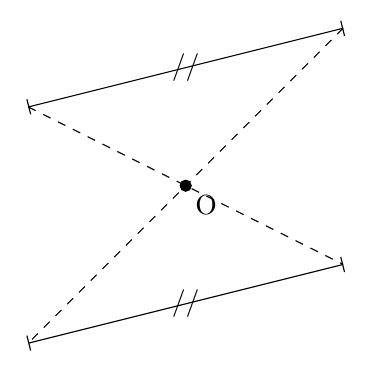
\begin{tikzpicture}
		\coordinate (O) at (0,0);
		\coordinate (A) at (-2,1);
		\coordinate (B) at (2,2);
		\coordinate[rotate around={180:(O)}] (A_sym) at (A);
		\coordinate[rotate around={180:(O)}] (B_sym) at (B);

		\draw[fill] (O) circle (2pt) node[anchor=north west] {O};

		\draw[|-|] (A) -- node {//} (B);
		\draw[|-|] (A_sym) -- node {//} (B_sym);
		\draw[dashed] (A) -- (A_sym);
		\draw[dashed] (B) -- (B_sym);
	\end{tikzpicture}
\end{cours}

\begin{cours}
	Deux figures symétriques par rapport à un point ont exactement la même forme : on dit que \myuline{la symétrie centrale conserve les angles}.
\end{cours}

\end{document}